%%%%%%%%%%%%%%%%%%%%%%%%%%%%%%%%%%%%%%%%%%%%%%%%%%%%%%%%%%%%%%%%%%%%%%%%%%%%
%% Trim Size : 11in x 8.5in
%% Text Area : 9.6in (include Runningheads) x 7in
%% ws-jai.tex, 26 April 2012
%% Tex file to use with ws-jai.cls written in Latex2E.
%% The content, structure, format and layout of this style file is the
%% property of World Scientific Publishing Co. Pte. Ltd.
%%%%%%%%%%%%%%%%%%%%%%%%%%%%%%%%%%%%%%%%%%%%%%%%%%%%%%%%%%%%%%%%%%%%%%%%%%%%
%%

%\documentclass[draft]{ws-jai}
\documentclass{ws-jai}
\usepackage[flushleft]{threeparttable}
\begin{document}

\catchline{}{}{}{}{} % Publisher's Area please ignore

\markboth{Bunch O people}{Analysis of robustness of BINGO optics.}

\title{Analysis of Robustness of BINGO optics.}

\author{First Author$^{2}$, Second Author$^{3}$, Third Author$^{3}$ and Fourth Author$^{4}$}

\address{
$^{2}$Department, University Name, City, State ZIP/Zone, Country, fauthor@university.com\\
$^{3}$Group, Company, Address, City, State ZIP/Zone, Country\\
$^{4}$Group, Company, Address, City, State ZIP/Zone, Country, fauthor@company.com
}

\maketitle

\corres{$^{2}$Corresponding author.}

\begin{history}
\received{(to be inserted by publisher)};
\revised{(to be inserted by publisher)};
\accepted{(to be inserted by publisher)};
\end{history}

\begin{abstract}
The abstract should summarize the context, content and conclusions
of the paper. It should not contain any references or displayed
equations. Typeset the abstract in 8~pt Times Roman with
baselineskip of 10 pt, making an indentation of 1.6~cm on the left
and right margins.
\end{abstract}

\keywords{Keyword 1; keyword 2; keyword 3.}

\section{The Main Text}
\noindent Contributions are to be in English. Authors are
encouraged to have their contribution checked for grammar.
American spelling should be used. Abbreviations are allowed but
should be spelt out in full when first used. Integers ten and
below are to be spelt out. Italicize foreign language phrases
({\it e.g.}~Latin, French).

\section{Major Headings}
Major headings should be typeset in boldface, with the first
letter of important words capitalized.

\subsection{Subheadings}
Subheadings should be typeset in bold italics, with the first
letter of first word capitalized and the section number in
boldface.

\subsubsection{Sub-subheadings}
Typeset in italics (section number to be in roman) and capitalize
the first letter of the first word only.

\subsection{Numbering and spacing}
Sections, subsections and sub-subsections are numbered with Arabic
numerals. Use double spacing after major and subheadings, and
single spacing after sub-subheadings.

\section{Illustrations and Photographs}
Figures are to be inserted in the text nearest their
first reference. Please send one set of originals with copies. If the
publisher is required to reduce the figures, ensure that the
figures (including lettering and numbers) are large enough to be
clearly seen after reduction.

\begin{figure}[h]
\begin{center}
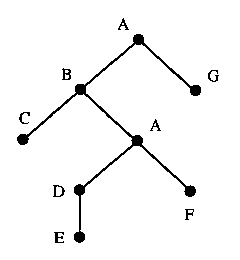
\includegraphics{jaif1} %100 percent
\end{center}
\caption{Labeled tree {\it T}.}
\label{aba:fig1}
\end{figure}

\begin{rotatefigure}
\begin{center}
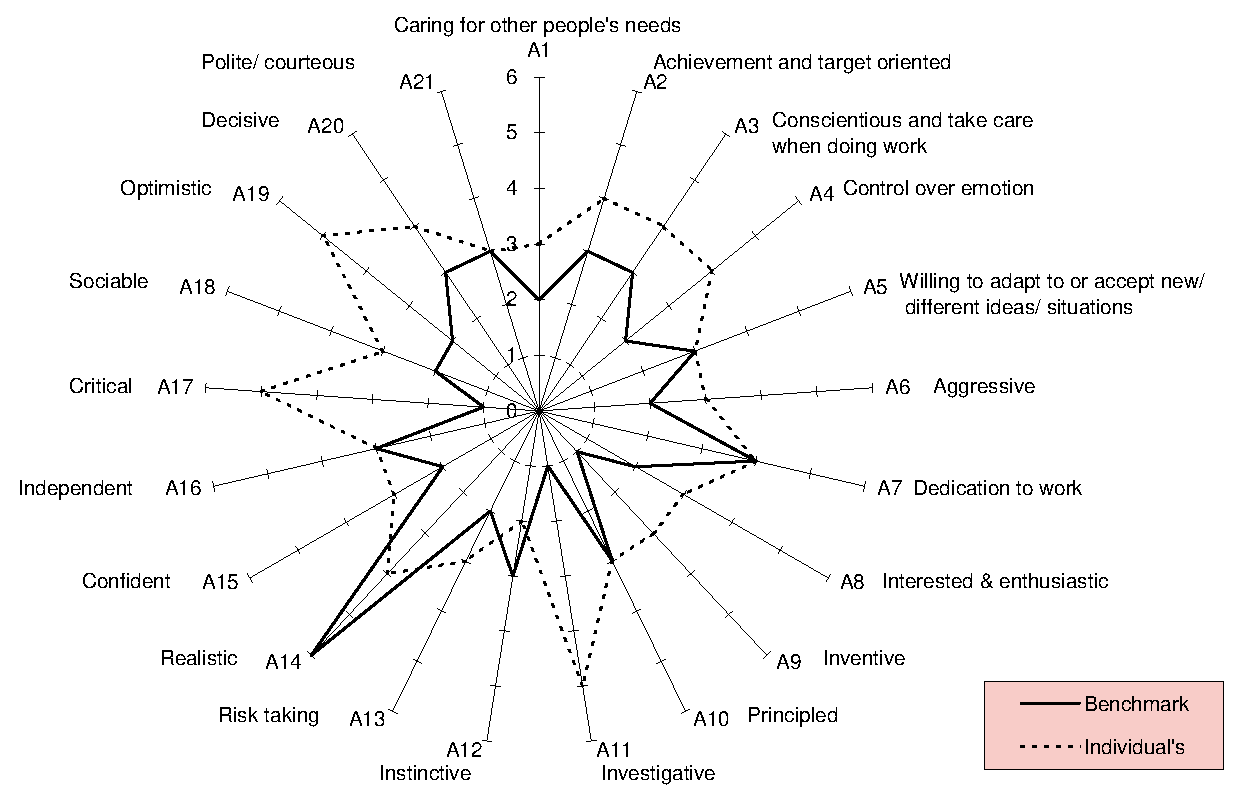
\includegraphics[width=7in]{jaif2}
\end{center}
\caption{The bifurcating response curves of system
$\alpha=0.5, \beta=1.8; \delta=0.2, \gamma=0$: (a)
$\mu=-1.3$; and (b) $\mu=0.3$.}
\label{aba:fig2}
\end{rotatefigure}

Figures are to be sequentially numbered with Arabic
numerals. The caption must be placed below the figure. For those
figures with multiple parts which appear on different pages, it is
best to place the full caption below the first part, and have
{\it e.g.}~``Fig.~1 ({\it continued})'' below the last part. Typeset in
9 pt Times Roman with baselineskip of 11 pt. Use double spacing
between a caption and the text that follows immediately.
Previously published material must be accompanied by written
permission from the author and publisher.

\section*{Note Added}
A note can be added before Acknowledgments.

\section*{Acknowledgments}
This part should come before References. Funding information may also be included here.


\bibliographystyle{ws-jai}

\bibliography{sample}
\end{document}
